\documentclass[11pt,twocolumn]{article}

\usepackage{cmap} % Generates ToUnicode mapping tables for PDF text extraction
% --- Core packages ---
\usepackage[utf8]{inputenc}
\usepackage[T1]{fontenc}
\usepackage{lmodern}  % Latin Modern fonts: provides proper ToUnicode CMaps for PDF text extraction
\usepackage{amsmath,amssymb,amsfonts,amsthm}
\usepackage{mathtools}
\usepackage{bm}
\usepackage{graphicx}
\usepackage{booktabs}
\usepackage{tabularx}
\usepackage{multirow}
\usepackage{enumitem}
\usepackage{hyperref}
\usepackage{cleveref}
\usepackage{xcolor}
\usepackage{microtype}
\usepackage{algorithm}
\usepackage{algpseudocode}
\usepackage[margin=0.85in]{geometry}
\usepackage{caption}
\usepackage{subcaption}
\usepackage{float}
\usepackage{listings}
\usepackage{stfloats} % Stabilizes two-column floats and prevents text overlap anomalies

% --- Code listing style (ensures reliable glyph rendering for copy-paste) ---
\lstset{
  language=Python,
  basicstyle=\footnotesize\ttfamily,
  columns=flexible,
  keepspaces=true,
  breaklines=true,
  frame=none,
  xleftmargin=1em,
  showstringspaces=false,
  commentstyle=\itshape\color{gray},
}

\hypersetup{
  colorlinks=true,
  linkcolor=blue!70!black,
  citecolor=green!50!black,
  urlcolor=blue!60!black
}

\newcommand{\simplex}{\mathcal{S}}
\newcommand{\closure}{\mathcal{C}}
\newcommand{\R}{\mathbb{R}}
\newcommand{\N}{\mathcal{N}}

\title{Automated Code-Guided Chart Synthesis and Visual Degradation:\\
A Unified Framework for Multimodal Document Parsing\\
and Visual Reasoning Benchmarks}

\author{
  Gabriel S Stuart\thanks{Correspondence: gabrielst13@outlook.com}
}

\date{}

\begin{document}
\maketitle

% ============================================================
%  ABSTRACT
% ============================================================
\begin{abstract}
Modern multimodal large language models (MLLMs) and visual document parsing networks require massive, 
structurally diverse datasets to decode complex relationships between text, categorical structures, and graphical primitives.
Crowdsourced human annotation pipelines are non-scalable, labor-intensive, and prone to low-level spatial coordinate errors.
This paper introduces an automated, code-guided chart synthesis framework that connects explicit mathematical data-generation engines directly to high-level graphical layout compilers.
Operating across specialized scientific and business domains, the system generates bar, line, box plot, heatmap, pie, histogram, scatter, and area charts while extracting pixel-perfect ground-truth coordinates, visual scene graphs, and adaptive multi-keypoint pose schemas.
To minimize the visual domain gap between idealized digital graphics and real-world scanned documents, vector outputs are passed through a comprehensive post-rendering physical degradation pipeline executing perspective homography transforms, multi-channel chromatic aberrations, spatial blur kernels, and non-uniform lighting fields.
The framework draws on Tufte's~\cite{tufte2001} design philosophy of graphical integrity by minimizing non-data ink and analyzing coordinate-space prerequisites for non-linear scale verification.
\end{abstract}

\smallskip
\noindent\textbf{Keywords:} Code-Guided Synthesis, Multimodal Large Language Models, Visual Encodings, Computational Visualization, Image Degradation Frameworks, Spatial Ground Truth.

% ============================================================
%  1. INTRODUCTION
% ============================================================
\section{Introduction}\label{sec:intro}

Interpretation of data visualizations constitutes a critical benchmark for evaluating visual reasoning in machine learning, requiring networks to integrate textual OCR, structural orientation tracking, coordinate scale matching, and multi-step quantitative reasoning.
Traditional computer vision datasets rely on crowdsourced manual annotations---a paradigm inherently non-scalable and susceptible to bounding-box inaccuracies that severely disrupt training of networks designed to extract precise numerical values from high-density charts.
Code-guided visualization synthesis pipelines circumvent these constraints by programmatically linking data frames to visual styles, establishing a direct, automated channel between data tables and graphic components.
This approach underpins modern vision-language benchmarks: ChartNet~\cite{kondic2026chartnet} and ChartMaster~\cite{liu2026chartmaster} convert raw databases into executable rendering configurations, while ChartGemma~\cite{masry2024chartgemma} combines web-harvested data tables with programmatic charts for instruction tuning.
Similarly, ChartGen~\cite{kondic2025chartgen} scales chart understanding via synthetic code-guided generators. Other benchmarks like ChartQAPro~\cite{masry2025chartqapro} and EncQA~\cite{han2026encqa} investigate visual encodings and complex multi-step reasoning over high-density layouts.
Synthesize Step-by-Step~\cite{li2024synthesize} deploys template-driven code abstractions for generating logically sound question--answer pairs, and DreamStruct~\cite{peng2024dreamstruct} demonstrates initializing visual datasets from structural specifications.
In parallel, Chart2Text-Enriched~\cite{suh2025chart2text} benchmarks models on fine-grained and context-aware chart summarization.

Training exclusively on pristine digital vectors introduces a significant domain gap.
Real-world documents encounter print-and-scan alterations, hand-held camera perspective warping, lens defocusing, and sensor noise.
Synthetic pipelines must therefore integrate post-rendering degradation operations that simulate physical paper defects while dynamically keeping all internal spatial coordinate logs updated. 
A comparative summary of standard visual chart synthesis pipelines is presented in Table~\ref{tab:pipeline_comparison}.

\begin{table}[htbp]
\centering
\caption{Comparison of synthetic chart generation pipelines.}\label{tab:pipeline_comparison}
\small
\begin{tabularx}{\columnwidth}{l c c c c}
\toprule
\textbf{Pipeline} & \textbf{Degrad.} & \textbf{Coord. Prop.} & \textbf{Keypoints} & \textbf{Profiles} \\
\midrule
ChartNet~\cite{kondic2026chartnet} & -- & -- & -- & General \\
ChartGemma~\cite{masry2024chartgemma} & -- & -- & -- & Web \\
ChartGen~\cite{kondic2025chartgen} & Limited & -- & -- & General \\
\textbf{Ours} & \textbf{Full} & \textbf{Warp/Rot} & \textbf{5/51-pt} & Sci/Biz \\
\bottomrule
\end{tabularx}
\end{table}

This article details a comprehensive, code-guided visualization synthesis and image degradation architecture.
We examine how Tufte's~\cite{tufte2001} design constraints---specifically the minimization of non-data ink through themes such as \texttt{minimal} and \texttt{prism}---execute across high-level statistical plotting architectures including Matplotlib~\cite{hunter2007matplotlib} and Seaborn~\cite{waskom2021seaborn}.
We establish a formal mathematical record of the system's design parameters, analyze the coordinate-space prerequisite transformations required for non-linear scale verification, and document the geometric warp profiles for building robust visual document reasoning benchmarks.

% ============================================================
%  2. PIPELINE ARCHITECTURE & DOMAIN TAXONOMY
% ============================================================
\section{Pipeline Architecture \& Domain Taxonomy}\label{sec:architecture}

The generation framework configures the chart rendering workspace through a unified configuration hierarchy, splitting variables across two structural application profiles to guarantee that categorical taxonomies, noise boundaries, and presentation themes mirror the distinct publishing rules of technical journals and corporate dashboards.

\subsection{The Scientific Profile}\label{sec:scientific}

The scientific profile emulates experimental measurements, biological assays, and clinical outcomes.
The text engine selects string parameters from an index of over 100 professional measurement combinations (\texttt{SCIENTIFIC\_DOMAIN\_DICT}), dynamically injecting axis labels such as \emph{Reads per million (RPM)}, \emph{Dissociation Constant ($K_{\text{d}}$, nM)}, \emph{Optical Density ($OD_{600}$)}, \emph{Molarity (mM)}, \emph{Fold Change}, and \emph{NMR Chemical Shift (ppm)}.
Categorical markers pull from authentic biological sequences: common oncogenes (TP53, BRCA1, BRCA2, EGFR, KRAS) and cellular pathways (PI3K-AKT, MAPK, WNT, Apoptosis).
The scientific profile enforces high-precision error bars, explicit statistical significance brackets, and highly skewed or zero-inflated continuous density structures to model realistic physical instrumentation baselines.

\subsection{The Business Profile}\label{sec:business}

The business profile emulates corporate analytics, performance indicators, and economic charts.
Text strings map enterprise metric taxonomies (\texttt{BUSINESS\_DOMAIN\_DICT}), utilizing combinations such as \emph{Monthly Active Users (MAU)}, \emph{Customer Lifetime Value (LTV~\$)}, \emph{Cost per Acquisition (CAC~\$)}, \emph{Net Promoter Score (NPS)}, and \emph{EBITDA~(\$)}.
Categorical labels draw from organizational records: specific product SKUs, subscription billing cycles, fulfillment timelines, and localized geographic sales regions.
Structurally, the business profile focuses on multi-component seasonal trends, exponential adoption constraints, market ceilings, and clean monochromatic or corporate-accented color layouts.

% ============================================================
%  3. MATHEMATICAL DATA GENERATION ENGINES
% ============================================================
\section{Mathematical Data Generation Engines}\label{sec:math}

Rather than utilizing flat uniform random variables, the framework draws continuous tracks from explicit mathematical equations parameterized to model realistic natural phenomena and business records.

\subsection{Dose--Response Curves (The Hill Equation)}\label{sec:hill}

Drug efficacy, chemical stimulus bounds, and cellular transitions across a range of log concentrations are modeled via a sigmoidal profile derived from the first-principles physiological model of Hill~\cite{hill1910dissociation}:
\begin{equation}\label{eq:hill}
  \text{data} = \text{baseline} + \frac{\text{max\_response} \mathbin{\text{-}} \text{baseline}}{1 + 10^{h(\text{ec50} \mathbin{\text{-}} \log_{\text{conc}})}},
\end{equation}
where concentration bounds range from pM to mM scales ($\log_{\text{conc}} \in [\text{-}10, \text{-}3]$), the inflection median scales as $\text{ec}_{50} \sim \mathcal{U}(\text{-}8.5, \text{-}4.5)$, and the cooperativity coefficient $h$ varies dynamically: $\mathcal{U}(0.7, 1.3)$ for standard single binding, $\mathcal{U}(1.3, 2.0)$ for cooperative transitions, and $\mathcal{U}(2.0, 3.5)$ for high-cooperativity profiles. This sigmoidal behavior conforms to the standard parameters of Hill's physiological model~\cite{hill1910dissociation}.

Measurement noise is non-uniform, scaling dynamically with the local slope via heteroscedastic error modeling. This is modeled following the clinical assay statistical processing methods of Rodbard~\cite{rodbard1974statistical}, which characterize non-uniform variance across concentration ranges to simulate realistic variance bounds for downstream models. The coefficient of variation peaks near the inflection thresholds where the response fraction $r_f$ varies dynamically, replicating physical immunoassay and bioassay behaviors:
\begin{align}
  \text{cv} &= 0.05 + 0.10\sqrt{r_f \cdot (1 \mathbin{\text{-}} r_f)}, \label{eq:cv}\\
  \text{noise} &\sim \N\!\bigl(0,\;(\text{data} \cdot \text{cv})^2\bigr), \label{eq:hill_noise}
\end{align}
where $r_f = \text{(data - baseline)/(max\_response - baseline)}$ denotes the response fraction.

\subsection{Biological \& Technical Replicates}\label{sec:replicates}

Variability across independent cell populations is replicated via an asymmetric log-normal distribution, prioritized over symmetric Gaussian noise. As shown by Limpert, Stahel, and Abbt~\cite{limpert2001lognormal}, biological replication error accumulates multiplicatively, resulting in highly skewed population distributions across physical biological systems:
\begin{align}
  \sigma &= \sqrt{\log_e\bigl(1 + \text{CV}_{\text{target}}^2\bigr)}, \label{eq:lognorm_sigma}\\
  \mu &= \log_e(\text{mean\_val}) \mathbin{\text{-}} 0.5\,\sigma^2, \label{eq:lognorm_mu}\\
  \text{data} &\sim \exp\bigl(\N(\mu, \sigma^2)\bigr). \label{eq:lognorm}
\end{align}

The target parameter $\text{CV}_{\text{target}}$ matches validated literature envelopes based on standard laboratory protocol error baselines from the Eli Lilly and NCATS immunoassay methods guidelines~\cite{lilly2012immunoassay}. These bounds constrain the generative noise envelopes to mimic real clinical laboratories, ensuring downstream models trained on these baselines acquire higher robustness to physical lab variations. The protocol-specific targets are summarized in Table~\ref{tab:cv_baselines}.

\begin{table*}[t]
\centering
\caption{Empirical CV Baseline Envelopes (verified against Eli Lilly~\cite{lilly2012immunoassay}).}\label{tab:cv_baselines}
\small
\begin{tabularx}{\textwidth}{l c X}
\toprule
\textbf{Assay Platform / Protocol} & \textbf{Empirical CV} & \textbf{Primary Physical Mechanism of Variation} \\
\midrule
Quantitative PCR (qPCR) & $5\% - 15\%$ & Amplification efficiency drift, micro-volume pipetting errors \\
Western Blot & $10\% - 25\%$ & Membrane binding variance, transfer efficiency fluctuations \\
Dynamic Cell Microplates & $15\% - 35\%$ & Ambient edge effects, localized evaporation, temperature gradients \\
\bottomrule
\end{tabularx}
\end{table*}

\subsection{Exponential Decay and Pharmacokinetic Clearance}\label{sec:decay}

Chemical clearance or radioactive isotope degradation is simulated across a temporal vector $t$:
\begin{align}
  \text{data} &= (\text{init} \mathbin{\text{-}} \text{baseline}) \cdot e^{\text{-}k \cdot t} + \text{baseline}, \label{eq:decay}\\
  k &= \frac{\log_e 2}{t_{1/2}}, \qquad t_{1/2} \in [0.5,\, 72]~\text{hours}. \label{eq:halflife}
\end{align}
A proportional error envelope overlays the sequence:
\begin{equation}\label{eq:decay_noise}
  \text{noise} \sim \N\bigl(0,\; (\text{data} \cdot 0.08 + 0.02 \cdot \text{max\_scale})^2\bigr).
\end{equation}

\subsection{Enzyme Kinetics (Michaelis--Menten)}\label{sec:mm}

Initial reaction velocities under varying substrate concentrations are modeled via the first-principles hyperbolic substrate velocity relationship of Michaelis and Menten~\cite{michaelis1913kinetik}:
\begin{equation}\label{eq:mm}
  \text{data} = \frac{V_{\max} \cdot [\text{S}]}{K_m + [\text{S}]},
\end{equation}
where $V_{\max}$ is the maximum velocity and $K_m$ the Michaelis constant. This formulation models initial velocity simulations matching thermodynamic kinetic constants, preventing unphysical or arbitrary curve trends in enzymatic assay charts. Measurement noise follows $\text{CV} \in [0.05, 0.15]$, consistent with analytical chemistry quality control bounds.

\subsection{Spectroscopy \& Chromatography Peaks}\label{sec:peaks}

Mass spectrometry or chromatography elution profiles are generated via a Gaussian peak model:
\begin{equation}\label{eq:gauss_peak}
  \text{data} = A \cdot \exp\!\biggl(-\frac{(x-\mu)^2}{2\sigma^2}\biggr) + \text{baseline}.
\end{equation}
According to the partition theory of Martin and Synge~\cite{martin1941new}, elution peaks in chromatographic columns follow Gaussian profiles due to multi-stage partitioning. This model provides physical validation for chromatography simulation, mapping analytical chemistry limits onto the visual parameters. Poisson-like photon counting noise replicates authentic instrument physics:
\begin{equation}\label{eq:poisson_noise}
  \text{noise} \sim \N\!\Bigl(0,\;\bigl(0.3\sqrt{|\text{data}-\text{baseline}|}\bigr)^2\Bigr).
\end{equation}

\subsection{Compositional Data Models (The Aitchison Simplex)}\label{sec:simplex}

Proportional tracking charts represent data bounded on the Aitchison Simplex $\simplex^D$ defined by Aitchison~\cite{aitchison1986statistical}:
\begin{equation}\label{eq:simplex}
  \simplex^D = \Bigl\{\mathbf{x} \in \R^D \;\Big|\; x_i > 0,\; x_1 + \dots + x_D = 1\Bigr\}.
\end{equation}
Aitchison's formulation defines the mathematical structures of simplex geometry, showing that proportional datasets require log-ratio transformations to avoid spurious correlations and prevent scale-dependent artifacts in compositional tracking charts.

\paragraph{Closure ($\closure$).} Projects any raw positive vector into the simplex:
\begin{equation}\label{eq:closure}
  \closure(\mathbf{x}) = \biggl[\frac{x_1}{\sum_k x_k},\;\frac{x_2}{\sum_k x_k},\;\ldots,\;\frac{x_D}{\sum_k x_k}\biggr].
\end{equation}

\paragraph{Perturbation ($\oplus$).} Compositional addition via component-wise multiplication followed by closure:
\begin{equation}\label{eq:perturbation}
  \mathbf{x} \oplus \mathbf{y} = \closure\bigl([x_1 y_1,\; x_2 y_2,\;\ldots,\; x_D y_D]\bigr).
\end{equation}

\paragraph{Power Transform ($\odot$).} Scalar multiplication on the simplex:
\begin{equation}\label{eq:power}
  \alpha \odot \mathbf{x} = \closure\bigl([x_1^\alpha,\; x_2^\alpha,\;\ldots,\; x_D^\alpha]\bigr).
\end{equation}

\paragraph{Aitchison Distance ($d_A$).} The log-ratio geometric distance, where $g(\mathbf{x}) = (\prod_i x_i)^{1/D}$:
\begin{equation}\label{eq:aitchison_dist}
  d_A(\mathbf{x}, \mathbf{y}) = \sqrt{\sum_{i=1}^D \left(\log_e\frac{x_i}{g(\mathbf{x})} - \log_e\frac{y_i}{g(\mathbf{y})}\right)^{\!2}}.
\end{equation}

\paragraph{Sampling Configurations.}
Slices ($D \in [3, 12]$) are generated via several methods:

\noindent\emph{Asymmetric Dirichlet:}
\begin{equation}\label{eq:dirichlet}
  f(\mathbf{x};\bm{\alpha}) = \frac{1}{\mathrm{B}(\bm{\alpha})}\prod_{i=1}^D x_i^{\alpha_i - 1},
\end{equation}
modified by an asymmetry trend factor ($\text{trend} \in [1.0-s,\;1.0+s]$, $s \in [0.0,\,1.5]$).

\noindent\emph{Stick-Breaking Process:} Configured following the constructive definition of Sethuraman~\cite{sethuraman1994constructive}:
\begin{equation}\label{eq:stickbreak}
  V_k \sim \text{Beta}(1, \gamma),\;\gamma \in [1.0,8.0];\quad x_k = V_k\!\prod_{j=1}^{k-1}(1 - V_j).
\end{equation}
This model is used for sequential sampling of simplex weights from Beta distributions, ensuring proportional allocations are mathematically consistent in stacked area and pie chart layouts.

\noindent\emph{Kummer--Dirichlet (Type~I Confluent) Sampling:}
Compositions are generated by drawing latent components $\mathbf{z}$ from independent standard Gamma distributions on the positive orthant $\R_+^D$:
\begin{equation}\label{eq:kdga_raw}
  g(\mathbf{z}) \propto \biggl(\prod_{i=1}^D z_i^{\alpha_i - 1}\biggr)\exp\biggl(-\sum_{i=1}^D z_i\biggr),\quad \mathbf{z} \in \R_+^D.
\end{equation}
To introduce asymmetry and scale-dependent skewness, each realized component is tilted via the non-linear algebraic transformation $w_i = z_i e^{-\lambda z_i}$ before projection onto $\simplex^D$:
\begin{equation}\label{eq:kdga_closure}
  \mathbf{x} = \closure\!\bigl([z_1 e^{-\lambda z_1},\;\dots,\;z_D e^{-\lambda z_D}]\bigr).
\end{equation}
This transformation is based on the Kummer-Dirichlet innovations of Makgai, Bekker, and Arashi~\cite{makgai2021compositional}. Since it is non-linear, it avoids scaling cancellation under the closure operator, generating highly flexible, skewed compositional data profiles containing outliers. The parameter $\lambda \in [-3, 3]$ controls the intensity of this asymmetric deformation; setting $\lambda = 0$ yields $w_i = z_i$, recovering the standard Dirichlet distribution on $\simplex^D$.

\paragraph{Entropy-Loss Tail Aggregation.}
When slices exceed a threshold ($\text{max\_slices}=5$), low-weight components are collapsed into an ``Other'' category governed by Shannon entropy:
\begin{align}
  H(\mathbf{x}) &= -\sum_{i=1}^D x_i \log_2 x_i, \label{eq:entropy}\\
  \Delta H &= H(\mathbf{x}_{\text{orig}}) - H(\mathbf{x}_{\text{agg}}). \label{eq:entropy_loss}
\end{align}
If $\Delta H > 0.5$, consolidation terminates to preserve fine-grained structural data.

\subsection{Zero-Inflated Profiles for Histograms}\label{sec:zeroinflated}

Histogram observation pools ($N \in [300, 1200]$) are sampled across continuous and zero-inflated frameworks, drawing on single-cell genomics methodologies like MAST~\cite{finak2015mast}:

\noindent\emph{Gaussian Mixture Model (GMM):}
\begin{equation}\label{eq:gmm}
  f(x) = \sum_{k=1}^K w_k \cdot \frac{1}{\sigma_k\sqrt{2\pi}}\exp\biggl(-\frac{(x-\mu_k)^2}{2\sigma_k^2}\biggr),
\end{equation}
where $K \in [2,4]$ and weights $\mathbf{w}$ follow a uniform Dirichlet.

\noindent\emph{Weibull Distribution:}
\begin{equation}\label{eq:weibull}
  f(x) = \frac{c}{\lambda}\Bigl(\frac{x}{\lambda}\Bigr)^{c-1}\exp\biggl(-\Bigl(\frac{x}{\lambda}\Bigr)^c\biggr),\; c \in [0.8, 2.5].
\end{equation}

\noindent\emph{Zero-Inflated Gaussian (ZIG):} Bounded by zero-inflation thresholds:
\begin{equation}\label{eq:zig}
  X_i = \begin{cases}
    0 & \text{w.p. } \pi,\\
    \N(\mu,\sigma^2) & \text{w.p. } 1-\pi,
  \end{cases}\quad \pi \in [0.2, 0.6].
\end{equation}
The Zero-Inflated Gaussian model (Hurdle-normal) handles high-density zeros alongside continuous distributions, representing biological dropouts and detection limits as characterized in single-cell genomics frameworks like MAST~\cite{finak2015mast}.

\subsection{Scatter Trend and Clustered Models}\label{sec:scatter}

Scatter tracks are mapped against target $R^2$ bounds, following correlation and covariance models based on Pearson~\cite{pearson1897mathematical}:

\noindent\emph{Linear Core:}
\begin{align}
  \mathbf{y}_{\text{perf}} &= m(\mathbf{x}-\bar{x}) + c, \label{eq:scatter_linear}\\
  \sigma_{\text{noise}}^2 &= \sigma_{\mathbf{y}_{\text{perf}}}^2 \cdot \frac{1-R^2}{R^2}, \label{eq:scatter_noise}\\
  y_i &= y_{\text{perf},i} + \N(0,\;\sigma_{\text{noise}}^2). \label{eq:scatter_final}
\end{align}
This formulation maps linear cores and non-linear tracks against targeted $R^2$ coefficients to prevent arbitrary, unrepresentative data structures.

\noindent\emph{Nonlinear Tracks:} Quadratic ($y = ax^2 + bx + c$), exponential ($y = a\exp(bx/\text{scale}) + c$), or logarithmic ($y = a\log_e(x+1)+c$) matrices with proportional CV noise ($\text{CV}_{\text{noise}} \in [0.08, 0.15]$).

\noindent\emph{Bivariate Multicluster Profiles:}
$K \in [2,3,4]$ clusters are generated via multivariate normals:
\begin{align}
  N_k &= \max\bigl(5,\;\lfloor N/K \rfloor + \mathcal{U}\{-3,3\}\bigr), \label{eq:cluster_size}\\
  \bm{\Sigma}_k &= \begin{bmatrix} \sigma_{xx} & \sigma_{xy}\\ \sigma_{xy} & \sigma_{yy}\end{bmatrix},\quad \rho \in [-0.5,\,0.5], \label{eq:cluster_cov}\\
  \mathbf{P}_{i,k} &\sim \N_2(\bm{\mu}_k,\;\bm{\Sigma}_k). \label{eq:cluster_sample}
\end{align}

\paragraph{Note on Business-Domain Data Models.}
In the business profile, synthetic data generation models are deployed to simulate multi-dimensional transaction ledgers and corporate performance metrics.
These business-domain generators build upon financial synthetic data generation techniques reviewed in Meldrum et al.~\cite{meldrum2025newmoney} to capture multi-component seasonal waveforms and power-law Pareto distributions.

\subsection{Multi-Component Seasonality \& Trend}\label{sec:seasonal}

Macroeconomic timelines and consumer trends are simulated across fiscal calendars:
\begin{equation}\label{eq:seasonal}
  \text{data} = b + s \cdot x + \sum_{m}\bigl[a_m \cos(f_m x + \phi_m)\bigr],
\end{equation}
where the sub-component matrix $m$ concurrently evaluates annual periods ($f = 2\pi/12$) and quarterly cycles ($f = 2\pi/3$), and noise variance expands proportionally during peak seasonal waves.

\subsection{Saturated Exponential Growth}\label{sec:satgrowth}

User adoption curves are bounded by an explicit logistic carrying capacity ceiling:
\begin{equation}\label{eq:satgrowth}
  \text{raw} = y_0 \cdot e^{g \cdot t}, \quad \text{data} = \text{raw} / (1 + \text{raw}/C),
\end{equation}
where $C$ denotes the carrying capacity.

\subsection{Pareto Distributions}\label{sec:pareto}

Disparities across discrete operational brackets are sampled via a power-law Pareto distribution:
\begin{equation}\label{eq:pareto}
  \text{data} \sim \text{Pareto}(\alpha,\, x_m), \quad \alpha \in [1.05,\, 2.5].
\end{equation}

% ============================================================
%  4. VISUAL LAYOUT GENERATION & GEOMETRY SYNTHESIS
% ============================================================
\section{Visual Layout Generation \& Geometry Synthesis}\label{sec:layout}

The rendering engine converts data tables into layout components, adjusting orientations and geometries based on structural series densities.
To evaluate model capability in code generation and visual mimicking, benchmarks like ChartMimic~\cite{yang2025chartmimic} and StarVector~\cite{rodriguez2025starvector} assess how well MLLMs can reconstruct vector layouts from visual prompts.
This structural evaluation is further aided by functional generation trees, such as the Chain of Functions~\cite{wang2025chainoffunctions} pipeline.
Figure~\ref{fig:chart_gallery} showcases the aesthetic variety and structural layouts across the eight primary programmatic chart types supported by the synthesis framework.

\begin{figure*}[t]
  \centering
  \begin{subfigure}[b]{0.24\textwidth}
    \centering
    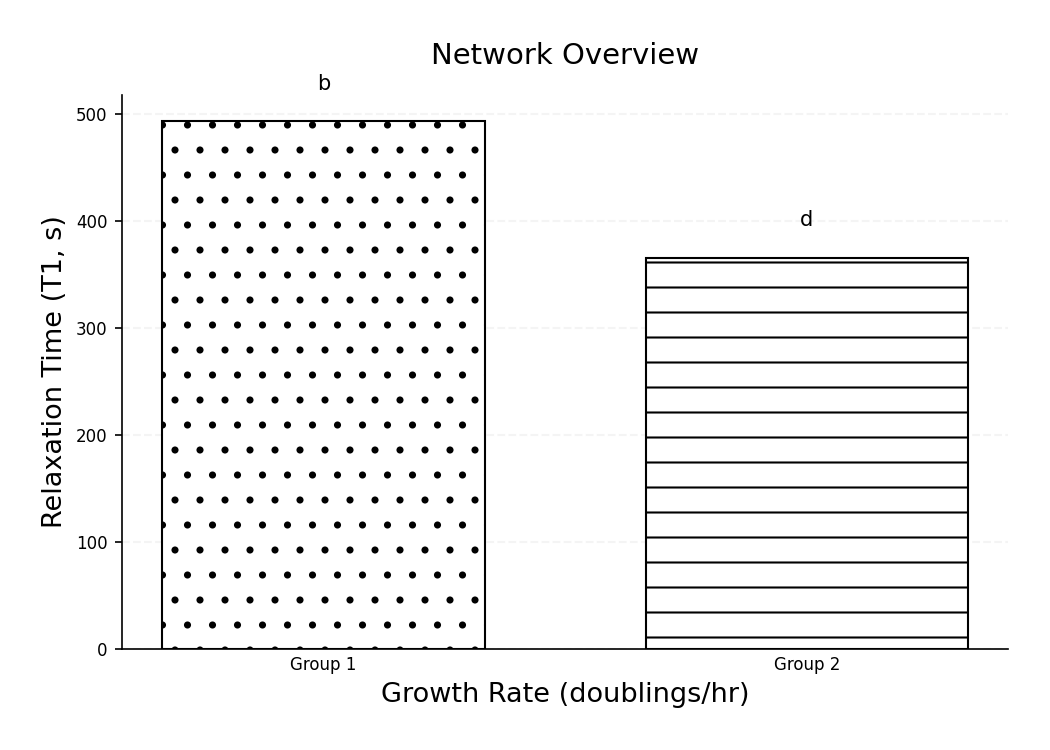
\includegraphics[width=\textwidth]{figures/fig_bar.png}
    \caption{Bar Chart}
    \label{fig:chart_bar}
  \end{subfigure}
  \hfill
  \begin{subfigure}[b]{0.24\textwidth}
    \centering
    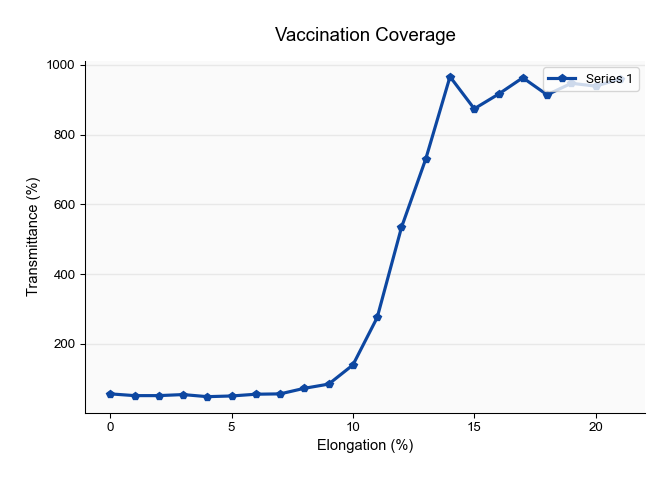
\includegraphics[width=\textwidth]{figures/fig_line.png}
    \caption{Line Chart}
    \label{fig:chart_line}
  \end{subfigure}
  \hfill
  \begin{subfigure}[b]{0.24\textwidth}
    \centering
    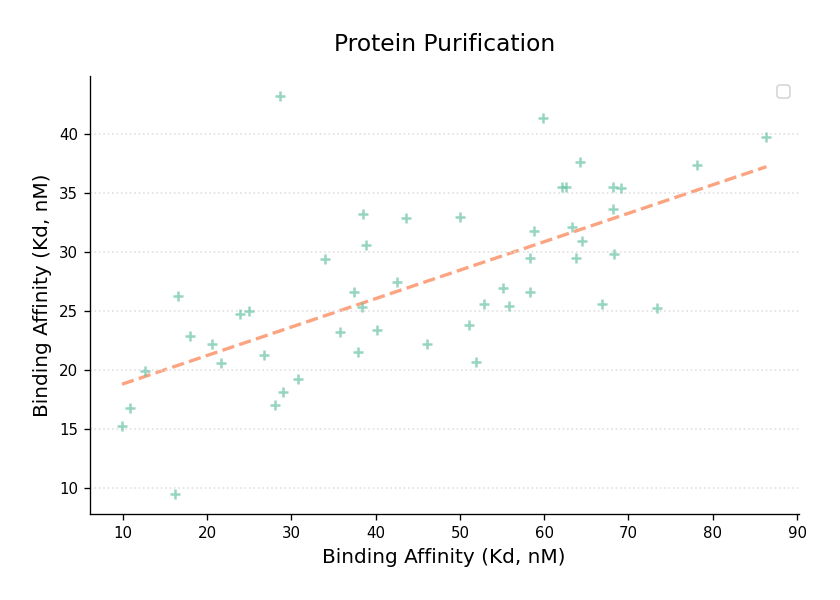
\includegraphics[width=\textwidth]{figures/fig_scatter.png}
    \caption{Scatter Chart}
    \label{fig:chart_scatter}
  \end{subfigure}
  \hfill
  \begin{subfigure}[b]{0.24\textwidth}
    \centering
    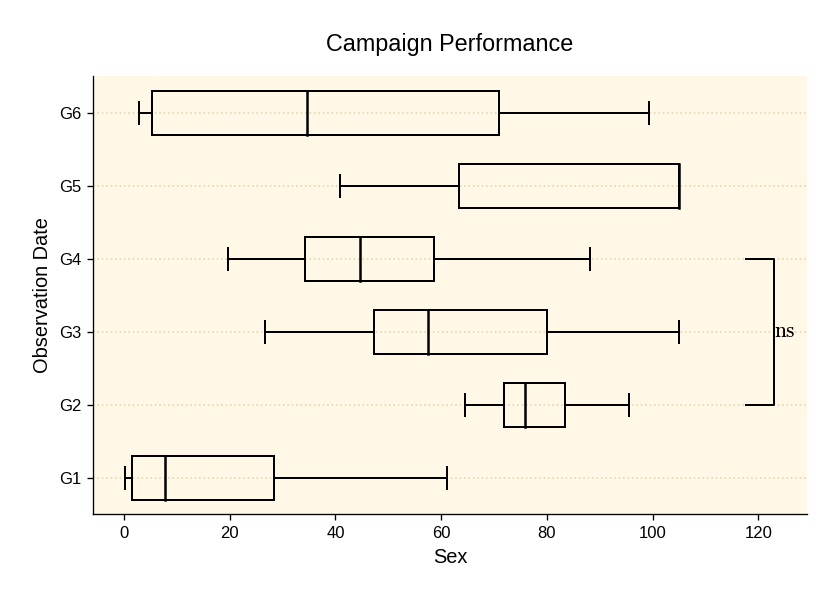
\includegraphics[width=\textwidth]{figures/fig_box.png}
    \caption{Box Plot}
    \label{fig:chart_box}
  \end{subfigure}
  \vskip\baselineskip
  \begin{subfigure}[b]{0.24\textwidth}
    \centering
    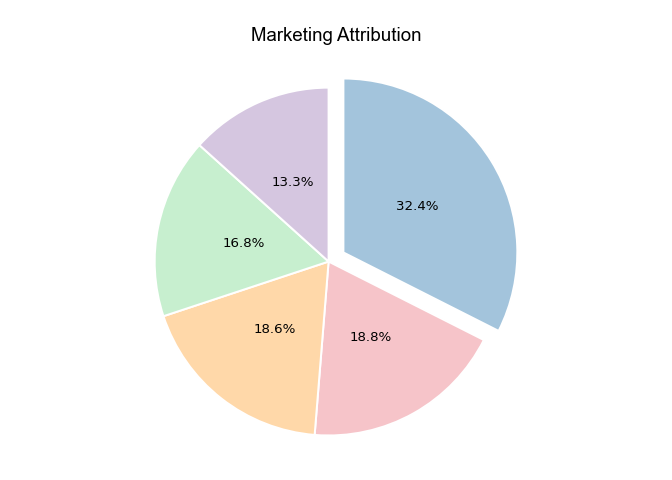
\includegraphics[width=\textwidth]{figures/fig_pie.png}
    \caption{Pie Chart}
    \label{fig:chart_pie}
  \end{subfigure}
  \hfill
  \begin{subfigure}[b]{0.24\textwidth}
    \centering
    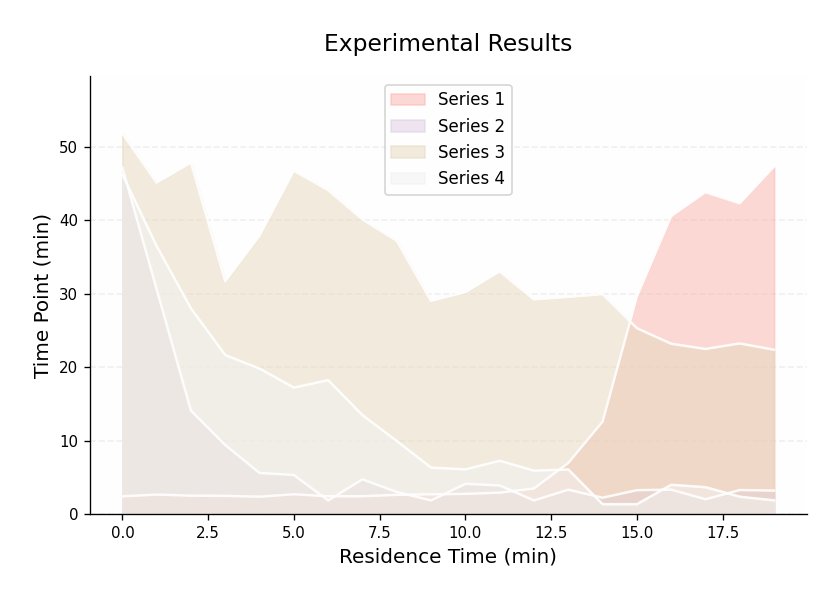
\includegraphics[width=\textwidth]{figures/fig_area.png}
    \caption{Area Chart}
    \label{fig:chart_area}
  \end{subfigure}
  \hfill
  \begin{subfigure}[b]{0.24\textwidth}
    \centering
    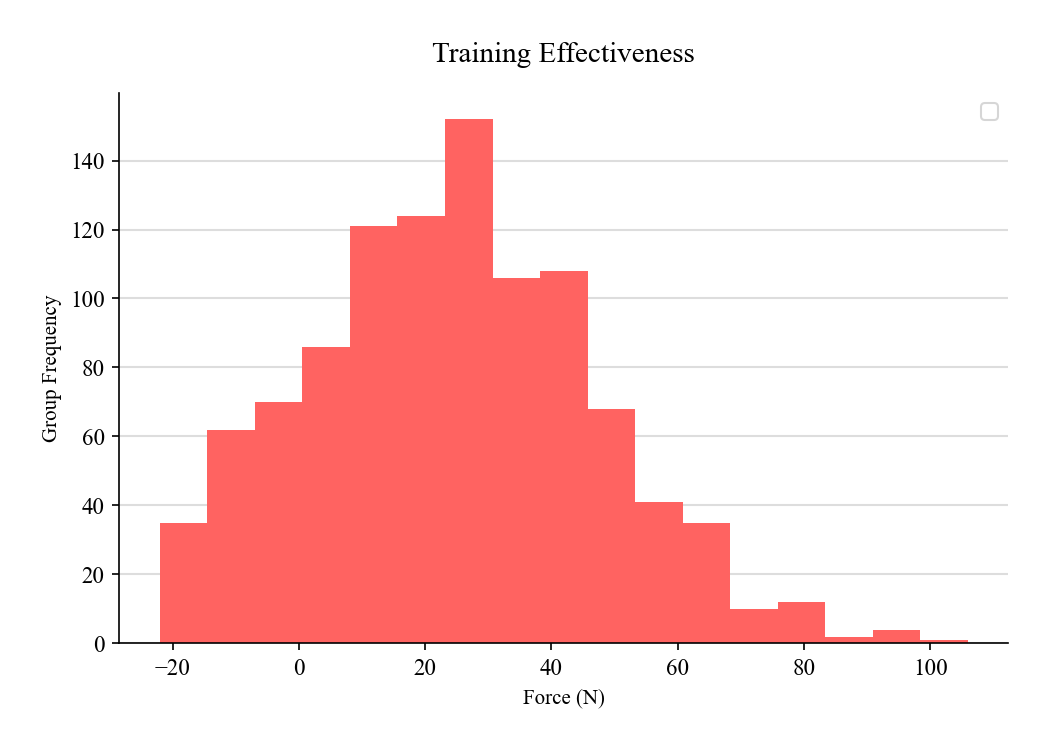
\includegraphics[width=\textwidth]{figures/fig_histogram.png}
    \caption{Histogram}
    \label{fig:chart_histogram}
  \end{subfigure}
  \hfill
  \begin{subfigure}[b]{0.24\textwidth}
    \centering
    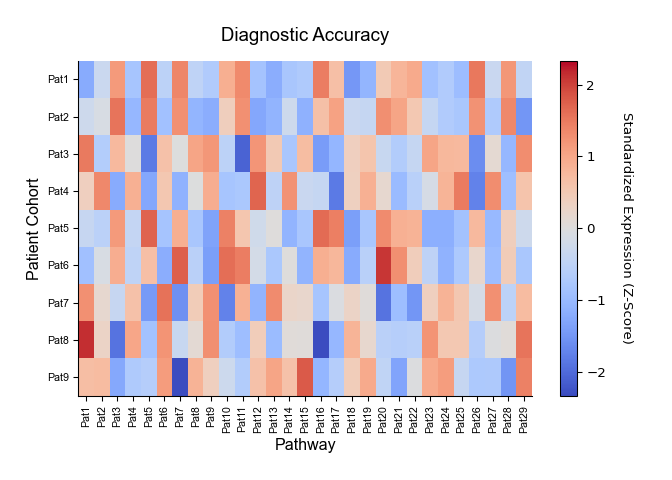
\includegraphics[width=\textwidth]{figures/fig_heatmap.png}
    \caption{Heatmap}
    \label{fig:chart_heatmap}
  \end{subfigure}
  \caption{Aesthetic variety and layout configurations across the eight primary programmatic chart types supported by the synthesis framework.}
  \label{fig:chart_gallery}
\end{figure*}

\subsection{Dimensional Configurations \& Layout Strategies}\label{sec:configs}

\paragraph{Primary Value Axis.} Switches between vertical and horizontal alignments when category lists exceed 6 groups to preserve label legibility.

\paragraph{Dual Y-Axis Scaling.} Maps distinct datasets onto identical category axes with independent left ($Y_1$) and right ($Y_2$) value scales.

\paragraph{Side-by-Side Grouping.} Arranges multiple series sequentially across categories using an indexed categorical displacement width ($\pm\text{width}/2$).

\paragraph{Stacked Segments.} The baseline coordinate vector for stacked layer $n$ resolves from the preceding cumulative total:
\begin{equation}\label{eq:stacked_bottom}
  \text{bottom}_n = \sum_{i=1}^{n-1} \text{height}_i.
\end{equation}
This cumulative stacking relies on the rendering mechanisms of Matplotlib~\cite{hunter2007matplotlib} to ensure geometric consistency under coordinate transformation matrices.

\paragraph{Area Chart Stacking Modes.} Three modes are supported: Overlapping ($\alpha=0.5$, filled from zero baseline), Stacked ($\alpha=0.7$, cumulative sequential layering), and Percentage/Normalized:
\begin{equation}\label{eq:pct_norm}
  y_{k,j} = \frac{y_{\text{raw},k,j}}{\sum_{i=0}^{K-1} y_{\text{raw},i,j} + \epsilon}\times 100.0.
\end{equation}

\paragraph{Hatch Textures.} Geometric patterns (\texttt{none}~= hollow, \texttt{..}~= dotted stipple, \texttt{//}~= diagonal stripes, \texttt{xxxx}~= crossed mesh) are mapped onto patches to retain readability in monochromatic or grayscale domains.

\paragraph{Statistical Significance Overlays.} Step-wise connecting lines drawn over targeted bar pairs, with horizontal beam clearance:
\begin{equation}\label{eq:sig_level}
  \text{level} = \max(\text{envelope})\cdot(1 + p),\quad p \in [0.10,\,0.20].
\end{equation}

\subsection{Bounding Box Resolution and Element Parsing}\label{sec:bbox}

\paragraph{Box Plot Schema (\texttt{CLASS\_MAP\_BOX}).}
The full 10-class contiguous index map ($\{0,\ldots,9\}$) includes generic element classes (\texttt{chart}~=~0, \texttt{axis\_title}~=~2, \texttt{significance\_marker}~=~3, \texttt{legend}~=~5, \texttt{chart\_title}~=~6, \texttt{axis\_labels}~=~8) shared across chart types.
The four box-plot-specific structural classes are:
\begin{itemize}[nosep]
  \item \texttt{box} (Class~1): IQR boundaries ($\text{IQR} = Q_3 - Q_1$).
  \item \texttt{range\_indicator} (Class~4): Union of upper/lower whiskers extending to $1.5\times\text{IQR}$.
  \item \texttt{median\_line} (Class~7): 50th percentile segment.
  A mandatory 3-pixel structural padding layer is applied because single line primitives return zero-area boundaries in raw display buffers.
  \item \texttt{outlier} (Class~9): Points beyond whisker thresholds.
\end{itemize}

\paragraph{Heatmap QuadMesh Parsing.}
For each row $i$ and column $j$, grid vertices are extracted:
\begin{equation}\label{eq:quad_corners}
  \text{Corners} = \bigl[\mathbf{c}_{i,j},\;\mathbf{c}_{i+1,j},\;\mathbf{c}_{i+1,j+1},\;\mathbf{c}_{i,j+1}\bigr].
\end{equation}
Grid vertices pass through \texttt{ax.transData.transform} to yield absolute canvas coordinates, normalized to $[0,1]$ for YOLO exports. Standard spatial translation transforms from Matplotlib~\cite{hunter2007matplotlib} map these arrays directly onto pixel coordinates, ensuring coordinate ground truth for heatmap cell grids. Auxiliary color bars are isolated by aspect ratio filtering ($w/h < 0.3$ vertical, $>3.0$ horizontal).

\subsection{Coordinate Pose Mapping \& Resampling Loops}\label{sec:pose}

\subsubsection{The 5-Keypoint Schema (Pie Charts)}\label{sec:5kpt}

Wedge paths are mapped to a 5-point geometry (\texttt{CLASS\_MAP\_PIE\_POSE}) based on the coordinate alignment schemas for high-level plotting utilities in Seaborn~\cite{waskom2021seaborn}. For exploded slices, the center shifts radially:
\begin{equation}\label{eq:wedge_center}
  \mathbf{c}_{\text{wedge}} = \bigl[\text{explode}\cdot\cos\theta_{\text{mid}},\;\text{explode}\cdot\sin\theta_{\text{mid}}\bigr].
\end{equation}
Intermediate arc coordinates sample at one-third and two-thirds of the angular span:
\begin{equation}\label{eq:arc_interp}
  \theta_{\text{int1}} = \theta_1 + \frac{\theta_2-\theta_1}{3},\quad \theta_{\text{int2}} = \theta_1 + \frac{2(\theta_2-\theta_1)}{3}.
\end{equation}
The 5 keypoints in display pixel space are indexed as follows: $\mathbf{k}_0$ is the wedge center, $\mathbf{k}_1$ and $\mathbf{k}_2$ correspond to the start and end angles of the wedge arc ($\theta_1$, $\theta_2$), and $\mathbf{k}_3$, $\mathbf{k}_4$ correspond to the interpolated interior positions ($\theta_{\text{int1}}$, $\theta_{\text{int2}}$):
\begin{align}
  \mathbf{k}_0 &= [x_c,\; y_c] + \mathbf{c}_{\text{wedge}}, \label{eq:k0}\\
  \mathbf{k}_n &= [x_c + r\cos\theta_n,\; y_c + r\sin\theta_n] + \mathbf{c}_{\text{wedge}}, \quad n \in \{1,2,3,4\}, \label{eq:kn}
\end{align}
where $\theta_1$, $\theta_2$ are the start and end angles of the wedge, $\theta_3 \coloneqq \theta_{\text{int1}}$, and $\theta_4 \coloneqq \theta_{\text{int2}} $.

% ============================================================
%  5. AESTHETIC THEMES & POST-RENDERING DEGRADATION
% ============================================================
\section{Aesthetic Themes \& Post-Rendering Degradation Mechanics}\label{sec:themes}

The pipeline decouples visual aesthetics into distinct declarative themes and publication presets before passing images through a post-rendering degradation framework.

\subsection{Thematic \& Publication Presets}\label{sec:presets}

The style engine (\texttt{themes.py}) configures canvas backdrops, grid visibility, line thicknesses, and typography classes.
Standard styles include:
\begin{itemize}[nosep]
  \item \textbf{excel}: Light-gray background (\texttt{\#F2F2F2}), thick solid white grids ($1.5\,$pt).
  \item \textbf{ggplot}: Dark-gray backdrop (\texttt{\#EBEBEB}), white grids, hidden outer spines.
  \item \textbf{prism}: White background, outward-pointing ticks, sparse dotted grid (\texttt{\#E0E0E0}).
  \item \textbf{retro}: Warm cream canvas (\texttt{\#FFF8E7}), Georgia serif fonts.
\end{itemize}

Rigid publication configurations (\texttt{PUBLICATION\_THEMES}) match peer-reviewed journal constraints:

\begin{table}[h!]
\centering
\caption{Publication preset configurations.}\label{tab:pub_presets}
\small
\begin{tabular}{l @{\hspace{1.2em}} c @{\hspace{1.2em}} c @{\hspace{1.2em}} c @{\hspace{1.2em}} c @{\hspace{1.2em}} c}
\toprule
\textbf{Preset} & \textbf{Size (in)} & \textbf{DPI} & \textbf{Font} & \textbf{Spine} & \textbf{Line}\\
\midrule
\texttt{nature}  & $3.3\!\times\!2.4$ & 300 & 7\,pt & 0.5\,pt & 0.5\,pt\\
\texttt{science} & $3.5\!\times\!2.5$ & 300 & 6\,pt & 0.75\,pt & 0.75\,pt\\
\texttt{cell}    & $6.5\!\times\!4.0$ & 300 & 8\,pt & 0.6\,pt & 0.6\,pt\\
\texttt{lancet}  & $7.0\!\times\!4.5$ & 300 & 8\,pt & 0.8\,pt & 0.8\,pt\\
\texttt{nanotech} & $3.2\!\times\!2.4$ & 600 & 7\,pt & 0.5\,pt & 0.6\,pt\\
\bottomrule
\end{tabular}
\end{table}

\subsection{Post-Rendering Image Degradation Filters}\label{sec:degradation}

Once compiled in vector format, images pass through a multi-tiered degradation pipeline implemented in \texttt{effects.py}.
The study of dynamic chart understanding and interactive action execution is further explored in benchmarks like ChartAct~\cite{zhou2026chartact}, which assess model performance in executing sequential actions over rendered visual canvases.
Figure~\ref{fig:degradation_comparison} illustrates a comparison between a clean programmatic rendering and its degraded counterpart after undergoing the multi-tiered degradation pipeline.

\begin{figure*}[t]
  \centering
  \begin{subfigure}[b]{0.48\textwidth}
    \centering
    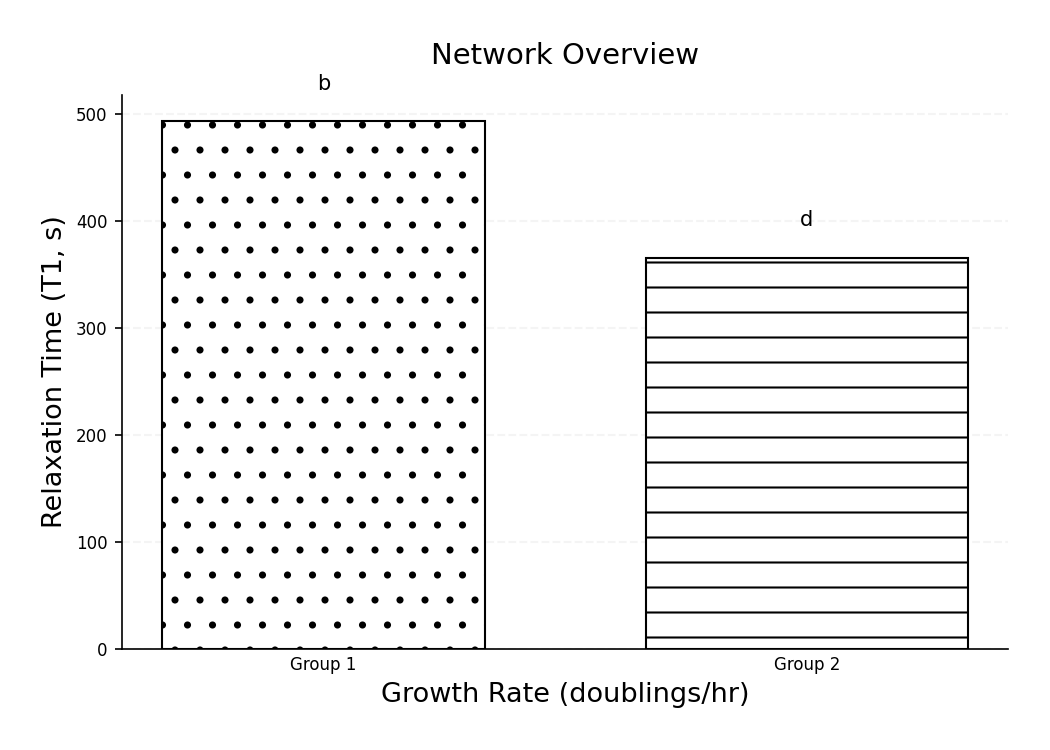
\includegraphics[width=\textwidth]{figures/fig_bar.png}
    \caption{Clean digital vector rendering.}
    \label{fig:degrad_clean}
  \end{subfigure}
  \hfill
  \begin{subfigure}[b]{0.48\textwidth}
    \centering
    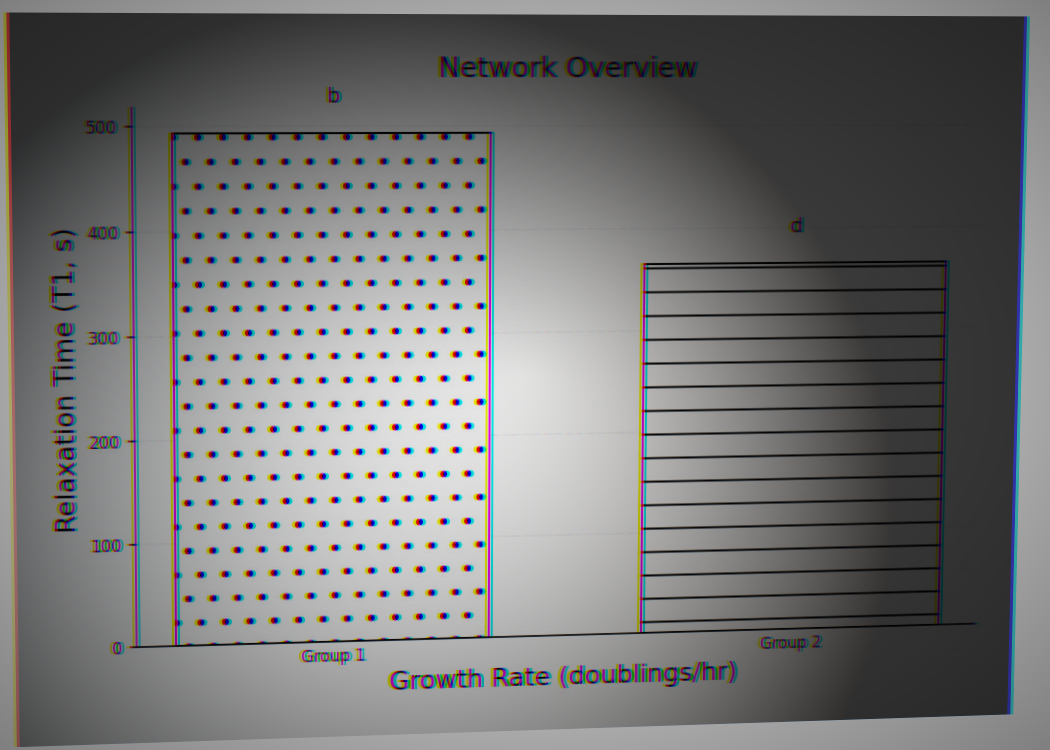
\includegraphics[width=\textwidth]{figures/fig_bar_degraded.png}
    \caption{Degraded canvas following the post-rendering pipeline.}
    \label{fig:degrad_dirty}
  \end{subfigure}
  \caption{Comparison of a clean digital rendering with a degraded document image passed through the post-rendering visual degradation pipeline (simulating scanner streaks, perspective warping, chromatic aberration, sensor noise, and uneven lighting).}
  \label{fig:degradation_comparison}
\end{figure*}

\subsubsection{General Realism Filters}\label{sec:general_filters}

General realism filters simulate physical sensor noise and optics degradation following the standard image processing formulations of Gonzalez and Woods~\cite{gonzalez2018digital}.

\paragraph{Edge Color Normalization (\texttt{normalize\_edgecolor}).} Darkens internal patch colors in HSV space, utilizing the transformation models governing patch edges and fill values in Matplotlib~\cite{hunter2007matplotlib}:
\begin{align}\label{eq:edge_norm}
  V_{\text{new}} &= \max(0,\; V \times 0.6), \nonumber \\
  \text{Edge} &= \text{HSV\_to\_RGB}(H, S, V_{\text{new}}).
\end{align}

\paragraph{Additive White Gaussian Noise (\texttt{apply\_noise\_effect}).}
\begin{equation}\label{eq:awgn}
  I_{\text{noisy}}(x,y,c) = \text{clip}\!\bigl(I_{\text{raw}}(x,y,c) + \text{N}(0,\sigma^2),\; 0,\;255\bigr),
\end{equation}
where $\sigma \sim \mathcal{U}(2.0, 8.0)$.

\paragraph{Directional Motion Blur.} A custom convolution kernel $\mathbf{K}$ models scanner bar movement:
\begin{align}
  x_{\text{idx}} &= \lfloor c + (i-c)\cos\theta\rfloor, \label{eq:motion_idx_x}\\
  y_{\text{idx}} &= \lfloor c + (i-c)\sin\theta\rfloor, \label{eq:motion_idx_y}\\
  \mathbf{K}(y_{\text{idx}}, x_{\text{idx}}) &= 1.0,\quad \mathbf{K}_{\text{norm}} = \mathbf{K}\Big/\!\sum\mathbf{K}. \label{eq:motion_kernel}
\end{align}

\paragraph{Vignette Lighting Falloff (\texttt{apply\_vignette\_effect}).} Quadratic radial attenuation:
\begin{align}
  r(x,y) &= \sqrt{(x-x_c)^2+(y-y_c)^2}, \label{eq:vig_r}\\
  V(x,y) &= \text{clip}\!\biggl(1 - \Bigl(\frac{r}{r_{\max}}\Bigr)^{\!2},\; 0.3,\; 1.0\biggr), \label{eq:vig_V}\\
  I_{\text{final}} &= I \cdot V(x,y). \label{eq:vig_final}
\end{align}

\paragraph{Chromatic Aberration (\texttt{apply\_chromatic\_aberration\_effect}).} Chromatic aberration is modeled as spatial shifts and scaling differences across RGB channels following Boult and Wolberg~\cite{boult1992correcting}, simulating physical lens dispersion by shifting the Red and Blue channels in opposite directions ($\Delta x, \Delta y$) relative to Green:
\begin{align}
  I_R(x,y) &= I_R(x+\Delta x_r,\; y+\Delta y_r), \label{eq:chrom_r}\\
  I_B(x,y) &= I_B(x+\Delta x_b,\; y+\Delta y_b). \label{eq:chrom_b}
\end{align}

\paragraph{Uneven Lighting (\texttt{apply\_uneven\_lighting\_effect}).} Subtractive illumination mask simulating flash hotspots or directional ambient gradients across the canvas grid:
\begin{align}\label{eq:uneven_light}
  M_{\text{radial}}(x,y) &= 1 - \frac{d(x,y)}{\max(d)}\cdot\text{intensity}, \nonumber\\
  &\quad \text{intensity} \in [0,1].
\end{align}

\subsubsection{Resolution and Compression Simulation}\label{sec:resolution}

\paragraph{Camera Downsampling (\texttt{apply\_low\_res\_effect}).} Shrinks via bicubic interpolation and scales back via bilinear: $\text{scale} \sim \mathcal{U}(0.25, 0.60)$.

\paragraph{Pixelation (\texttt{apply\_pixelation\_effect}).} Bilinear downsampling followed by nearest-neighbor upsampling creates block artifacts.

\paragraph{Palette Quantization (\texttt{apply\_posterize\_effect}).} Constrains continuous color depths to $N \in \{16, 32, 64\}$ indexed palette entries.

\subsubsection{Document Scanning \& Physical Overlays}\label{sec:scanning}

\begin{itemize}[nosep]
  \item \textbf{Scanner Streaks}: Semi-transparent horizontal bands at randomized heights simulate dust on a sensor bed.
  \item \textbf{Document Misalignment}: Rotation $\theta \sim \mathcal{U}(-1^\circ, 1^\circ)$.
  \item \textbf{UI Chrome Wrappers}: Desktop browser frames or web tab search bars overlaid at canvas boundaries.
  \item \textbf{Watermarks}: Low-opacity diagonal text stamps (e.g., \textsc{confidential}, \textsc{draft}) at canvas center.
  \item \textbf{Mouse Cursor}: Vector pointer arrow injected at randomized coordinates.
\end{itemize}

\subsubsection{Selective OCR-Targeted Text Degradation}\label{sec:text_degrad}

The module \texttt{apply\_text\_degradation\_effect} isolates textual regions---titles, legends, axis values---directly from the active scene graph via \texttt{get\_window\_extent}.
Targeted blur and pixelation kernels are applied exclusively within these bounding areas, leaving coordinate data curves untouched, forcing data parsing networks to learn robust visual patterns.

\subsubsection{The Aesthetic--Quantitative Tension}\label{sec:tension}

Pixel-level filters (vignette, noise, aberration) do not alter the coordinate structure of underlying features.
However, document rotation (\texttt{apply\_scan\_rotation\_effect}) introduces a physical spatial transform. This is resolved by computing a 2D rotation matrix about the canvas center:
\begin{equation}\label{eq:rotation_matrix}
  \begin{bmatrix} x' \\ y' \end{bmatrix} = \begin{bmatrix} \cos\theta & \sin\theta \\ -\sin\theta & \cos\theta \end{bmatrix} \begin{bmatrix} x - x_c \\ y - y_c \end{bmatrix} + \begin{bmatrix} x_c \\ y_c \end{bmatrix},
\end{equation}
where $(x_c, y_c)$ is the canvas center. By propagating this transform into the pipeline's coordinate transformation steps (\texttt{transform\_steps}), the system dynamically rotates the ground-truth bounding boxes and multi-keypoint pose schemas to match the rotated pixel canvas.
A similar tension arises if hand-drawn sketch rendering modes (e.g., \texttt{plt.xkcd()}) are integrated, as sketch jitter introduces non-deterministic displacements of rendered elements relative to the extracted coordinates.

\subsection{Homography \& Perspective Warping Mechanics}\label{sec:homography}

The perspective transformation (\texttt{apply\_perspective\_warp\_effect}) maps original corner coordinates to randomized targets shifted inward:
\begin{equation}\label{eq:distortion}
  \Delta x = w \cdot d,\quad \Delta y = h \cdot d,\quad d = 0.08.
\end{equation}

The projection maps source $[x,y]^T$ to warped $[u,v]^T$ via a $3\!\times\!3$ perspective matrix, following the Direct Linear Transformation (DLT) photogrammetry method of Abdel-Aziz and Karara~\cite{abdelaziz1971direct}:
\begin{equation}\label{eq:proj_mat}
  \begin{bmatrix} u \\ v \\ 1\end{bmatrix} \sim
  \begin{bmatrix} h_1 & h_2 & h_3 \\ h_4 & h_5 & h_6 \\ h_7 & h_8 & 1\end{bmatrix}
  \begin{bmatrix} x \\ y \\ 1\end{bmatrix}.
\end{equation}
This maps the source coordinates to the projected targets in a continuous coordinate space.

The eight unknown parameters are solved by expanding four corner mappings into $A\mathbf{h} = \mathbf{b}$:
\begin{equation}\label{eq:homography_system}
  \left[\setlength{\arraycolsep}{3.5pt}\begin{array}{cccccccc}
    x_i & y_i & 1 & 0 & 0 & 0 & -u_i x_i & -u_i y_i\\
    0 & 0 & 0 & x_i & y_i & 1 & -v_i x_i & -v_i y_i
  \end{array}\right]
  \mathbf{h} = \begin{bmatrix} u_i \\ v_i\end{bmatrix}.
\end{equation}
The homography vector is solved via standard least-squares matrix inversion, as formulated in the DLT framework of Abdel-Aziz and Karara~\cite{abdelaziz1971direct}:
\begin{equation}\label{eq:ls_solve}
  \mathbf{h} = (A^\top A)^{-1} A^\top \mathbf{b}.
\end{equation}

The inverse matrix $H^{-1}$ is passed to the image processing engine for pixel interpolation.
When OpenCV is active, the system calls \texttt{cv2.getPerspectiveTransform} for deterministic $3\times3$ coordinate mapping, while falling back to the algebraic least-squares homography solver otherwise.
Ground-truth labels are projected via $H$:
\begin{equation}\label{eq:label_warp}
  \begin{bmatrix} x_w \\ y_w \\ w\end{bmatrix} = H \begin{bmatrix} x_o \\ y_o \\ 1\end{bmatrix},\quad
  \mathbf{p}_{\text{final}} = \biggl[\frac{x_w}{w},\;\frac{y_w}{w}\biggr].
\end{equation}

Cropping offsets from \texttt{apply\_clipping\_effect} apply additive coordinate adjustments:
\begin{equation}\label{eq:clip_adjust}
  x_{\text{adj}} = x_o + \Delta x,\quad y_{\text{adj}} = y_o + \Delta y.
\end{equation}

% ============================================================
%  6. EMPIRICAL EVALUATION & BENCHMARK VALIDATION
% ============================================================
\section{Empirical Evaluation \& Benchmark Validation}\label{sec:evaluation}

To validate the utility of the generated synthetic data for training visual parsing and document layout models, we construct a benchmarking suite and train specialized element detection networks across all eight supported chart types. 

\subsection{Experimental Setup}\label{sec:setup}

For each of the eight primary programmatic formats (bar, line, box plot, heatmap, pie, histogram, scatter, and area), a synthetic corpus is generated with randomized aesthetic themes, label configurations, and is subjected to the full suite of post-rendering degradation effects (directional motion blur, additive sensor noise, perspective homography warping, scanner streaks, and vignette lighting falloffs). Specifically, each heatmap model is trained on a corpus of 1,200/600 (75\%/25\%) train/validation images, while other graph formats utilize a corpus of 3,600/1,200 (75\%/25\%) train/validation images. The sole exception is the bar plot, which has 3,600/1,200 synthetic graphs supplemented by 351 real graphs annotated manually. The Hugging Face dataset\footnote{\url{https://huggingface.co/datasets/utcz/Plots/tree/main}} is a representative example of the generator.

Using this corpus, object detection and coordinate extraction networks are trained to locate chart primitives, axis labels, legends, titles, statistical significance markers, error bars, and specific structural shapes (e.g., box IQR blocks, outliers, and pie wedges). All models are trained on the latest YOLO11 model with varying epochs, running for at least 80 epochs each.

\subsection{Results and Performance Analysis}\label{sec:results}

Model performance is evaluated on the independent test sets using class-wise Average Precision (AP) and model-wide Mean Average Precision at an IoU threshold of 0.5 (mAP@0.5). Table~\ref{tab:evaluation_results} details the evaluation results across the ten benchmark models.

\begin{table*}[htbp]
\centering
\caption{Model element detection and structural layout parsing performance (mAP@0.5) on degraded synthetic chart datasets.}\label{tab:evaluation_results}
\small
\begin{tabularx}{\textwidth}{l X c c}
\toprule
\textbf{Model / Chart Type} & \textbf{Target Classes (Elements)} & \textbf{Class AP} & \textbf{Global mAP} \\
\midrule
Heatmap lattice & celldata\_label & 0.715, 0.995 & 0.855 \\
Heatmap Macro & chart, color\_bar\_region & 0.995, 0.995 & 0.995 \\
Heatmap Text & axis\_labels, axis\_title, chart\_title & 0.995, 0.995, 0.995 & 0.995 \\
Heatmap Color Bar & color\_bar, color\_bar\_label, color\_bar\_title & 0.995, 0.995, 0.994 & 0.995 \\
Bar Plot & bar, axis\_title, significance\_marker, error\_bar, legend, chart\_title, data\_label, axis\_labels & 0.992, 0.995, 0.942, 0.973, 0.987, 0.995, 0.935, 0.987 & 0.976 \\
Box Plot & box, axis\_title, significance\_marker, range\_indicator, chart\_title, median\_line, axis\_labels, outlier & 0.995, 0.995, 0.975, 0.995, 0.995, 0.715, 0.983, 0.701 & 0.919 \\
Histogram Plot & bar, axis\_title, chart\_title, data\_label, axis\_labels & 0.865, 0.989, 0.995, 0.901, 0.994 & 0.949 \\
Line Plot & data\_point, axis\_title, significance\_marker, legend, chart\_title, data\_label, axis\_labels & 0.895, 0.995, 0.236, 0.995, 0.995, 0.913, 0.982 & 0.859 \\
Pie Obj Plot & wedge, legend, chart\_title, data\_label, connector\_line & 0.986, 0.994, 0.995, 0.990, 0.905 & 0.974 \\
Scatter Plot & data\_point, axis\_title, chart\_title, axis\_labels & 0.914, 0.995, 0.995, 0.989 & 0.973 \\
\bottomrule
\end{tabularx}
\end{table*}

The baseline models demonstrate strong generalization capability on structural text elements (titles, axis titles, and legends) and macroscopic layouts (such as heatmap grids and color bars), consistently achieving AP values above 0.990. However, detection performance drops significantly on fine-grained, high-density elements under aggressive degradation, as discussed below.

% ============================================================
%  7. DISCUSSION
% ============================================================
\section{Discussion}\label{sec:discussion}

\subsection{Coordinate-Space Projection Boundaries (Lie Factor Prerequisites)}\label{sec:liefactor}

Tufte's~\cite{tufte2001} Lie Factor assumes graphic and data dimensions are measured within native linear coordinates:
\begin{equation}\label{eq:lie}
  \text{Lie Factor} = \frac{\Delta\text{Graphic Space}}{\Delta\text{Data Space}}.
\end{equation}
A na\"ive implementation computing graphical distance from raw canvas pixels yields systematic bias on non-linear scales. On a log axis spanning $10^0$ to $10^4$, bars spanning $[10^2,10^3]$ and $[10^3,10^4]$ occupy identical pixel distances, yet represent data-space changes of 900 vs.\ 9{,}000 units---a tenfold projection bias. Correct implementation requires passing coordinates through an inverted transformation matrix:
\begin{equation}\label{eq:lie_inv}
  \mathbf{p}_{\text{data}} = \mathbf{T}^{-1}\cdot\mathbf{p}_{\text{pixel}},\quad \mathbf{T} = \texttt{ax.transData.transform}.
\end{equation}
Mapping coordinate transformations across logarithmic scales using the inverse transformation matrix eliminates projection bias and prevents systematic overestimation of graphical features on logarithmic axes [13].

\subsection{Degradation Sensitivity in Fine-Grained Features}\label{sec:sensitivity}

As shown in Section~\ref{sec:results}, the detection performance of parsing networks exhibits varying degrees of sensitivity depending on the physical scale and complexity of the target element. 

While structural elements like boxes (0.995 AP) and chart backgrounds are highly robust, fine-grained details degrade severely under motion blur and perspective warping. In box plots, the median line (0.715 AP) and individual outlier points (0.701 AP) exhibit lower accuracy due to pixel-level occlusion under spatial blurring. 

Similarly, the statistical significance marker in line plots registers the lowest score in the benchmark suite (0.236 AP). This drop occurs because significance brackets are represented by narrow line segments topped with small text labels (e.g., \texttt{*} or \texttt{ns}); when subjected to perspective warping and downsampling, these fine graphic primitives lose their structural distinctiveness. This highlights a clear training boundary for document intelligence systems, demonstrating that visual degradation models successfully test the limits of spatial reasoning networks and force the need for higher-resolution visual encoders.

% ============================================================
%  8. CONCLUSION & FUTURE WORK
% ============================================================
\section{Conclusion \& Future Work}\label{sec:conclusion}

This paper has presented an automated, code-guided chart synthesis and physical degradation framework designed to bridge the data domain gap in multimodal document intelligence.
By mapping explicit continuous and compositional data models---the sigmoidal Hill equation, log-normal replicate variance, and the restricted Aitchison simplex---directly to structural graphic layouts, the framework provides a reliable alternative to manual annotation workflows.
Post-rendering image alterations simulate real-world document tracking and scanning artifacts through perspective homography solvers and 2D rotation matrix transformations while dynamically preserving bounding box limits and skeletal pose registers.

Future research will focus on integrating procedural vector layouts directly into active optimization loops of vision-language architectures via reinforcement learning. By querying the generation engines developed here, next-generation visual reasoning benchmarks can dynamically modulate layout complexity and artifact intensities to systematically expand model capabilities across highly degraded visual environments.

% ============================================================
%  REFERENCES
% ============================================================
\begin{thebibliography}{35}

\bibitem{abdelaziz1971direct}
Abdel-Aziz, Y. I., \& Karara, H. M. (1971).
\newblock Direct linear transformation from comparator coordinates into object space coordinates in close-range photogrammetry.
\newblock \emph{Proc.\ ASP/UI Symposium on Close-Range Photogrammetry}, pp.\ 1--18.

\bibitem{aitchison1986statistical}
Aitchison, J. (1986).
\newblock \emph{The Statistical Analysis of Compositional Data}.
\newblock Chapman \& Hall, London.

\bibitem{boult1992correcting}
Boult, T. E., \& Wolberg, G. (1992).
\newblock Correcting chromatic aberrations using image warping.
\newblock \emph{Proc.\ IEEE CVPR}, pp.\ 684--687.

\bibitem{finak2015mast}
Finak, G., McDavid, A., Yajima, M., Deng, K., Gersuk, V., Shalek, A. K., Slichter, C. K., Miller, H. W., McElrath, M. J., Prlic, M., Linsley, P. S., \& Gottardo, R. (2015).
\newblock MAST: a flexible statistical framework for assessing cell-specific differences in single-cell RNA-seq gene expression data.
\newblock \emph{Genome Biology}, 16, p.\ 278.

\bibitem{gonzalez2018digital}
Gonzalez, R. C., \& Woods, R. E. (2018).
\newblock \emph{Digital Image Processing} (4th ed.).
\newblock Pearson.

\bibitem{han2026encqa}
Han, S. et al. (2026).
\newblock EncQA: Benchmarking Vision-Language Models on Visual Encodings for Charts.
\newblock \emph{IEEE Transactions on Visualization and Computer Graphics} [Preprint/Early Access].

\bibitem{he2016resnet}
He, K., Zhang, X., Ren, S., \& Sun, J. (2016).
\newblock Deep residual learning for image recognition.
\newblock \emph{Proc.\ IEEE CVPR}, pp.\ 770--778.
\newblock DOI: 10.1109/CVPR.2016.90

\bibitem{hill1910dissociation}
Hill, A. V. (1910).
\newblock The possible effects of the aggregation of the molecules of haemoglobin on its dissociation curves.
\newblock \emph{The Journal of Physiology}, 40(1), pp.\ iv--vii.

\bibitem{hunter2007matplotlib}
Hunter, J.~D. (2007).
\newblock Matplotlib: A 2D graphics environment.
\newblock \emph{Computing in Science \& Engineering}, 9(3), pp.\ 90--95.
\newblock DOI: 10.1109/MCSE.2007.55

\bibitem{kondic2026chartnet}
Kondic, J. (2026).
\newblock ChartNet: A million-scale, high-quality multimodal dataset for robust chart understanding.
\newblock \emph{arXiv preprint arXiv:2603.27064}.

\bibitem{kondic2025chartgen}
Kondic, J. et al. (2025).
\newblock ChartGen: Scaling Chart Understanding Via Code-Guided Synthetic Chart Generation.
\newblock \emph{arXiv preprint arXiv:2507.02424}.

\bibitem{li2024synthesize}
Li, Z., Jasani, B., Tang, P., \& Ghadar, S. (2024).
\newblock Synthesize step-by-step: Tools, templates and LLMs as data generators for reasoning-based chart VQA.
\newblock \emph{Proc.\ IEEE/CVF CVPR}, pp.\ 13613--13623.
\newblock DOI: 10.1109/cvpr52733.2024.01292

\bibitem{lilly2012immunoassay}
Eli Lilly \& Company, \& National Center for Advancing Translational Sciences. (2012).
\newblock Immunoassay Methods.
\newblock In \emph{Assay Guidance Manual}. National Institutes of Health.

\bibitem{limpert2001lognormal}
Limpert, E., Stahel, W. A., \& Abbt, M. (2001).
\newblock Log-normal distributions across the sciences: Keys and clues.
\newblock \emph{BioScience}, 51(5), pp.\ 341--352.

\bibitem{liu2026chartmaster}
Liu, C. (2026).
\newblock ChartMaster: Boosting MLLMs for chart analysis through data, perception, and reasoning optimization.
\newblock \emph{OpenReview / ICLR} [Preprint/Early Access].

\bibitem{makgai2021compositional}
Makgai, S., Bekker, A., \& Arashi, M. (2021).
\newblock Compositional data modeling through Dirichlet innovations.
\newblock \emph{Mathematics}, 9(19), p.\ 2477.

\bibitem{martin1941new}
Martin, A. J. P., \& Synge, R. L. M. (1941).
\newblock A new form of chromatogram employing two liquid phases.
\newblock \emph{Biochemical Journal}, 35(12), pp.\ 1358--1368.

\bibitem{masry2024chartgemma}
Masry, A., Thakkar, M., Bajaj, A., Kartha, A., Hoque, E., \& Joty, S. (2024).
\newblock ChartGemma: Visual instruction-tuning for chart reasoning in the wild.
\newblock \emph{arXiv preprint arXiv:2407.04172}.

\bibitem{masry2025chartqapro}
Masry, A. et al. (2025).
\newblock ChartQAPro: A New Benchmark for Complex Chart Question Answering.
\newblock \emph{Findings of the Association for Computational Linguistics (ACL)}.

\bibitem{meldrum2025newmoney}
Meldrum, J., Suleiman, B., Rabhi, F., \& Alibasa, M.~J. (2025).
\newblock New money: A systematic review of synthetic data generation for finance.
\newblock \emph{arXiv preprint arXiv:2510.26076}.

\bibitem{michaelis1913kinetik}
Michaelis, L., \& Menten, M. L. (1913).
\newblock Die Kinetik der Invertinwirkung.
\newblock \emph{Biochemische Zeitschrift}, 49, pp.\ 333--369.

\bibitem{peng2024dreamstruct}
Peng, Y.-H., Huq, F., Jiang, Y., Wu, J., Li, X.~Y., Bigham, J.~P., \& Pavel, A. (2024).
\newblock DreamStruct: Understanding slides and user interfaces via synthetic data generation.
\newblock \emph{LNCS}, pp.\ 466--485.
\newblock DOI: 10.1007/978-3-031-72691-0\_26

\bibitem{pearson1897mathematical}
Pearson, K. (1897).
\newblock Mathematical contributions to the theory of evolution. On a form of spurious correlation which may arise when indices are used in the measurement of organs.
\newblock \emph{Proc.\ Royal Society of London}, 60, pp.\ 489--498.

\bibitem{rodriguez2025starvector}
Rodriguez, J. et al. (2025).
\newblock From Charts to Code: A Hierarchical Benchmark for Multimodal Models.
\newblock \emph{OpenReview / Structural Vision Workshop}.

\bibitem{rodbard1974statistical}
Rodbard, D. (1974).
\newblock Statistical quality control and routine data processing for radioimmunoassays and immunoradiometric assays.
\newblock \emph{Clinical Chemistry}, 20(10), pp.\ 1255--1270.

\bibitem{sethuraman1994constructive}
Sethuraman, J. (1994).
\newblock A constructive definition of Dirichlet priors.
\newblock \emph{Statistica Sinica}, 4(2), pp.\ 639--650.



\bibitem{suh2025chart2text}
Suh, S. et al. (2025).
\newblock Chart2Text-Enriched: Towards Fine-Grained and Context-Aware Chart Summarization.
\newblock \emph{IEEE Transactions on Visualization and Computer Graphics}.

\bibitem{tufte2001}
Tufte, E.~R. (2001).
\newblock \emph{The Visual Display of Quantitative Information} (2nd ed.).
\newblock Graphics Press, Cheshire, CT.
\newblock ISBN: 0-9613921-4-2

\bibitem{wang2025chainoffunctions}
Wang, X. et al. (2025).
\newblock Chain of Functions: A Programmatic Pipeline for Fine-Grained Chart Reasoning Data Generation.
\newblock \emph{arXiv / ACL Anthology}.

\bibitem{waskom2021seaborn}
Waskom, M.~L. (2021).
\newblock seaborn: statistical data visualization.
\newblock \emph{Journal of Open Source Software}, 6(60), p.\ 3021.
\newblock DOI: 10.21105/joss.03021

\bibitem{yang2025chartmimic}
Yang, Z. et al. (2025).
\newblock ChartMimic: Evaluating LMMs' Code Generation Elements via Visual Mimicking.
\newblock \emph{arXiv preprint arXiv:2501.03152}.

\bibitem{zhou2026chartact}
Zhou, M. et al. (2026).
\newblock ChartAct: A Benchmark for Dynamic Chart Understanding.
\newblock \emph{arXiv preprint arXiv:2605.26994} [Preprint/Early Access].

\end{thebibliography}

\end{document}